%
% Document template suitable for use as a latex master-file for masters
% thesis in University of Turku Laboratory of Electronics and Information
% Technology. Relies on itpackage.sty for additional definitions.
%
% Sami Nuuttila (samnuutt@utu.fi) 
%
% Last mod 11.6.2007:
%
% Some modifications between 2009-2016: Antti Hakkala (ajahak@utu.fi)
% 
% Why:
%  · No need for anyone to invent the wheel again. You can of course do that
%    if you wish - TeX'll even let you invent many different kinds of wheels
%  · That said, if you come up with a great new wheel I'd like to hear about 
%    it - it might even end up being used here 
% 
% Features:
%  · Proper page sizes as required by university guide for students:
%      · proper font sizes as well as linespacings
%      · proper size of margins
%  · Generic title page:
%      · \gentitle
%  · Generic abstract page(s):
%      · \begin{itabstract}{Keywords}
%          abstract text
%        \end{itabstract}
%      · \begin{ittiivis}...\end{ittiivis} provides finnish version
%         · ittiivis defaults to finnish so no need to issue 
%           \selectlanguage{finnish}
%      · total number of pages as well as total number of pages in appendices
%        are automagically handled
%  · Entry environment:
%      · \begin{entry}[widest label]
%          \item[1st label text] ...
%          \item[2nd label text] ...
%        \end{entry}
%      · the actual items are aligned to suit the widest label, which is
%        given as an argument to the environment
%  · Use of specific latex packages to ease in formatting the thesis:
%      · format table of contents to have bibliography shown as references
%        as well as other fixes           (tocbibind)
%      · enhanced verbatim handling       (sverb)
%      · source code inclusion            (listings)
%      · handling of headers and footers  (fancyhdr)
%
%      · consultation of the manuals of these packages is strongly
%        encouraged 
%
% Assumptions:
%  · itpackage.sty file is available 
%  · each chapter is as a separate file which is read in with e.g. \input
%   
% Miscellaneous:
%  · comments are welcome
%  · should a required package be missing see http://www.ctan.org/ 
%  · http://www.ctan.org/tex-archive/info/lshort/english/lshort.pdf
%
%%%%%%%%%%%%%%%%%%%%%%%%%%%%%%%%%%%%%%%%%%%%%%%%%%%%%%%%%%%%%%%%%%%%%%%%%%%

%%%%%%%%%%%%%%%%%%%%%%%%%%%%%%%%%%%%%%%%%%%%%%%%%%%%%%%%%%%%%%%%%%%%%%%%%%%
%
% load all required packages
%
%%%%%%%%%%%%%%%%%%%%%%%%%%%%%%%%%%%%%%%%%%%%%%%%%%%%%%%%%%%%%%%%%%%%%%%%%%%

% document is based on report class
\documentclass[a4paper,12pt]{report}

% load ams-packages for maths
\usepackage{amssymb,amsthm,amsmath}

% load babel-package for automatic hyphenation
\usepackage[english,finnish]{babel}
\usepackage[T1]{fontenc} % Tavutus ääkkösille
\usepackage[utf8]{inputenc}

% load graphicx package
%   · automagically select proper parameters depending on whether
%     we're running pdflatex or latex
%   · specify \includegraphics{file} without the file extension
%     (.eps /.pdf (/ .png / .jpeg / ...)), tex should select the proper file
%
\usepackage{ifpdf}
\usepackage{graphicx}
\usepackage[hyphens]{url} %URLit ehjänä perille
%% !!! NOTE: if you have old LaTeX distribution then you might need to
%% use the following
%% \newif\ifpdf
%% \ifx\pdfoutput\undefined
%%   \pdffalse
%% \else
%%   \pdfoutput=1
%%   \pdftrue
%% \fi
%% % if graphicx complains about option clash remove the [pdftex] option
%% \ifpdf
%%   \usepackage[pdftex]{graphicx}
%% \else
%%   \usepackage[dvips]{graphicx}
%% \fi


% load tocbibind package 
%   · do not include table of contents in itself
%   · convert the name of bibliography to references
\usepackage[nottoc]{tocbibind}
%\settocbibname{References}

% load sverb package
%   · enhanced handling of verbatim stuff; listing environment
%\usepackage{sverb}

% load listings package
%   · handle inclusion of source code
\usepackage{listings}
\usepackage{placeins}

\usepackage{xcolor} % for setting colors

% set the default code style
\lstset{
    frame=tb, % draw a frame at the top and bottom of the code block
    tabsize=4, % tab space width
    showstringspaces=false, % don't mark spaces in strings
    numbers=left, % display line numbers on the left
    commentstyle=\color{green}, % comment color
    keywordstyle=\color{blue}, % keyword color
    stringstyle=\color{red} % string color
}




% load fancyheaders package
%   · the actual headers and footers are set later
\usepackage{fancyhdr}

% load itpackage 
%   · additional defines and stuff
\usepackage{itpackage}

% Antin omat asetukset <3
\settocbibname{References}
\setcounter{tocdepth}{2}
\usepackage{lipsum}

% Jos (ja kun) TeX rikkoo tavutussääntöjä, kerro sille tässä miten homma tehdää oikein...

%\hyphenation{k{\"a}m-me-nen-j{\"a}l-ki}% sään-nön-mu-kai-nen hy-väk-syt-tä-vyys hy-väk-syn-näl-tään kier-ret-tä-vyy-del-tään mer-kit-tä-väs-ti bi-o-met-ri-sis-tä käyt-tö-oi-keu-den pyr-kii e-sit-tä-mi-nen mi-kä-li hyl-kää-mi-ses-tä bi-o-met-ri-seen}
 
%%%%%%%%%%%%%%%%%%%%%%%%%%%%%%%%%%%%%%%%%%%%%%%%%%%%%%%%%%%%%%%%%%%%%%%%%%%
%
% main document starts here
%
%%%%%%%%%%%%%%%%%%%%%%%%%%%%%%%%%%%%%%%%%%%%%%%%%%%%%%%%%%%%%%%%%%%%%%%%%%%
\begin{document}
%%% fill in your information below
\workinfo{Tijam Moradi and Oskari Vahala}
{SSNS project report}
{}
{} % Toinen tarkastaja, jätetään tyhjäksi kandityössä
{2019}
{November}
{}
%% set the type of your thesis (Diplomityö, TkK -tutkielma, etc.) below
\worktype{Type of thesis}{Arduino based test bed with XBee} 
%% set the laboratory or field of study
\deptinfo{Laboratory Name}{Communication Systems} % Tähän oppiaine, jonka alle työ kuuluu


% generate the title page 
\gentitle

% generate tiivistelma
%\begin{ittiivis}{Laita, tähän, lista, avainsanoista}

%\end{ittiivis}

% if your thesis is in english then this is also required (is it???)
%\begin{itabstract}{list, of, keywords}
%If your thesis is in english this might also be required???
%\end{itabstract}

% select language here (note that english also needs to set enclname)
\selectlanguage{english}
%\selectlanguage{english}\def\enclname{Appendices}

% empty pagestyle for table of contents etc. 
%
% the redefinition of plain style works also for 1st pages of chapters,
% which is the default in report class. Just state \thispagestyle{empty}
% after \chapter{something} if you want empty style for the 1st pages. 
%
\pagestyle{empty}
\fancypagestyle{plain}{
  \fancyhf{}
  \renewcommand{\headrulewidth}{0 pt}
}

% roman numbering for table of contents etc.
\pagenumbering{roman}

% insert table of contents, list of figures, list of tables
%
% setting the counter to zero effectively removes the page number from
% the toc, lof etc. entries in the toc since there is no roman numeral
% for zero ;-) (if you want them without numbering)
%
%\setcounter{page}{0}
%\tableofcontents
\clearpage
%\setcounter{page}{0}

% Lista kuvista
%\listoffigures 

\clearpage
%\setcounter{page}{0}

% Lista taulukoista
%\listoftables

% possibly insert 'list of acronyms'
%
%   · create a chapter called List Of Acronyms (or whatever), which
%     should contain all your acronym definitions, e.g. 
%     \chapter{List Of Acronyms} 
%   · the secnumdepth trickery is needed because acronyms are as a
%     standard chapter and we are faking '\listofacronyms'
%
%\setcounter{secnumdepth}{-1}
%\input{your acronym chapter's file name}
%\setcounter{secnumdepth}{2}


% setup page numbering, page counter, etc.
\startpages

%%%%%%%%%%%%%%%%%%%%%%%%%%%%%%%%%%%%%%%%%%%%%%%%%%%%%%%%%%%%%%%%%%%%%%%%%%%
%
% hi ho hi ho it's off to work we go....
%
% from now on you're on your own -- good luck!
%
% that is to say that the actual thesis should come here 
%
%%%%%%%%%%%%%%%%%%%%%%%%%%%%%%%%%%%%%%%%%%%%%%%%%%%%%%%%%%%%%%%%%%%%%%%%%%%

% Työn voi joko kirjoittaa tähän sellaisenaan...
\chapter{Introduction}

We had a task to build a sensor network to a warehouse. We thought that it would be right approach to monitor conditions on the warehouse using sensors that measures temperature and humidity. There is a possibility that the warehouse stores articles that needs to be stored in certain conditions. We also had one ultrasonic sensor that we used to keep track on the state of the large door of the warehouse. 

This project has the intention for us to learn about networking technologies right on low level. The project uses DIGI XBee S2D shields for communication. We have four sets of: Arduino, XBee shield, XBee transmitter, Sensor (either proximity or humidity + temperature).
Since the original documentation for the project requirements were ambiguous, we decided to make an implementation as close as possible. 

One of the four devices will be solely a base station. This base station will receive the data from other devices and forward it to USB serial for remote monitoring. We consider USB Serial is remote enough for this project, since we don’t have Bluetooth or WiFi shields to send data to cloud. The purpose of the project also is not to build something in the cloud but wireless secure networking on ground. 

The other four devices will have one of two sensors; temperature and humidity or proximity. Each device will read and process the data from the respective sensors. The processed data will then be sent to the base station for remote monitoring. The base station itself does not make use of a sensor since we have decided that its sole purpose is to gather the data and forward it in good telemetry. If we were to mix the base station with sensor logic there could be problems in future with scalability. 
The telemetry from the sensor devices is transferred to the base station with RPL IPv6 via mesh network. In this kind of scenario, we can have the devices more far away from the base station. 








\chapter{Network design}

On this project we used ZigBee network with XBEE S2D units. Network consists of a coordinator and three routers that work also as sensor nodes (figure \ref{fig:topology}). ZigBee is a low powered personal area network that is designed for low powered IOT devices. 
Sensor nodes are working as routers because we would place them on forklifts. It is possible for node to move around the storage unit. There is a possibility for a node to bee too far away from the coordinator that the communication would not be possible without using another node as a relay node. That is the reason why our implementation does not have ‘real’ end nodes. Power management is also harder to implement, because routers are not allowed to sleep or if they sleep, it would have to be synchronized. 


\begin{figure}[h!]
\caption{Topology of the network}
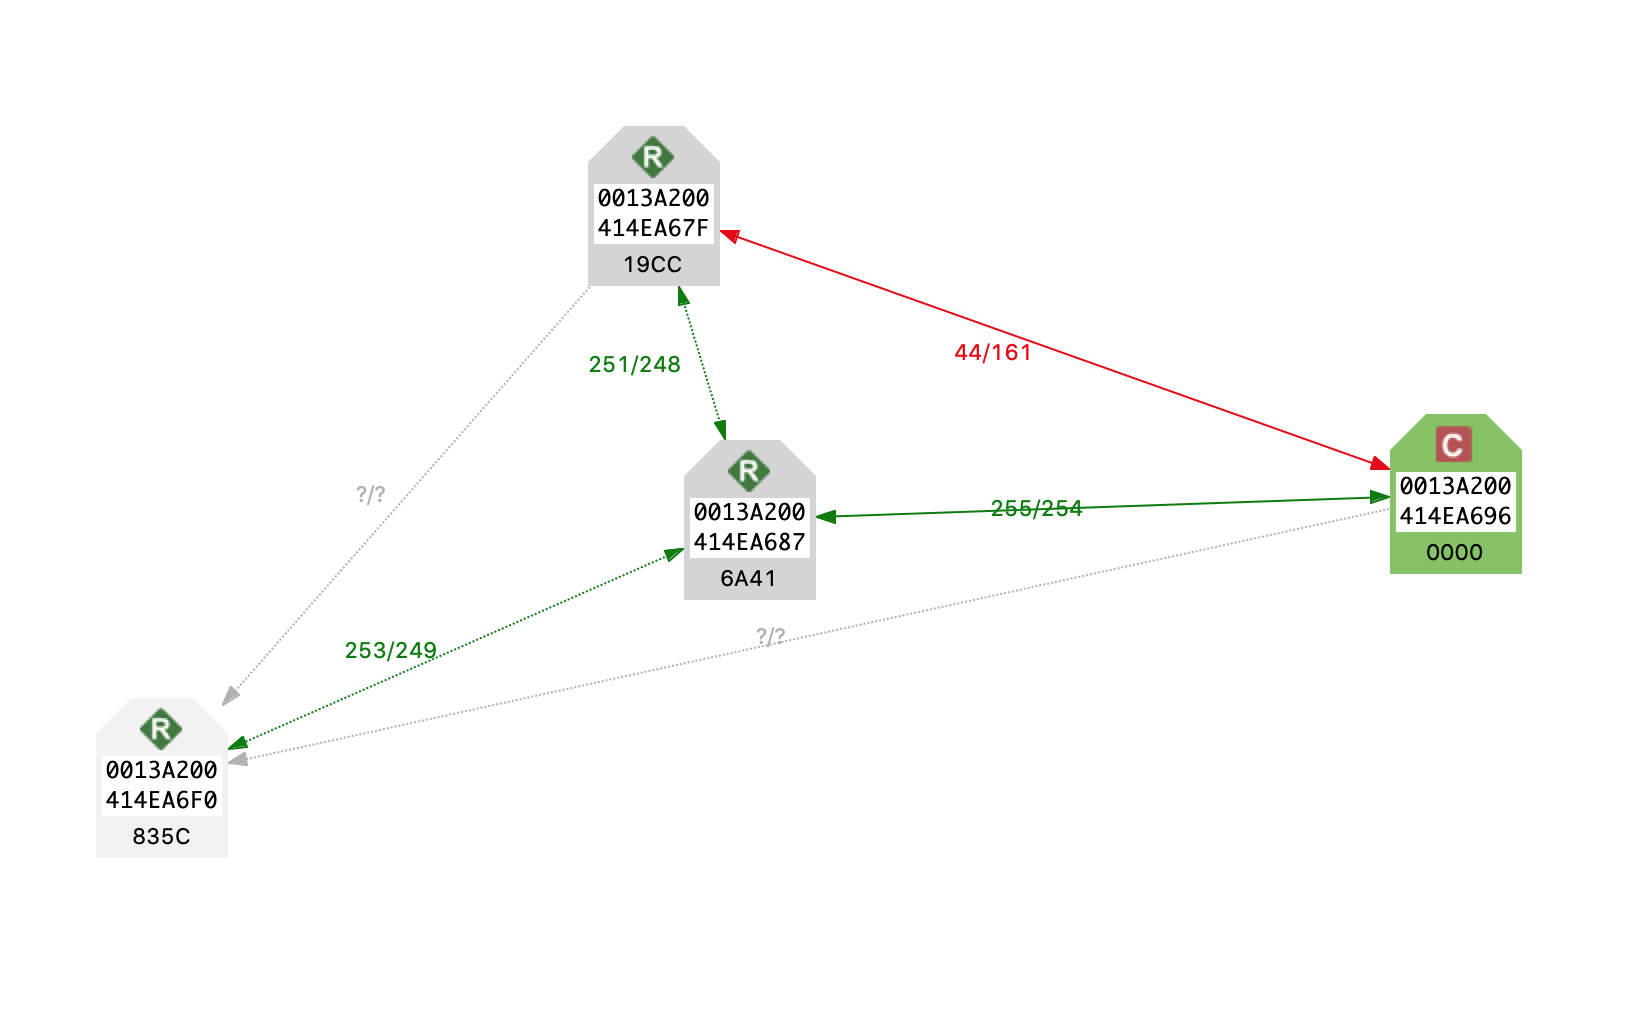
\includegraphics[width=\textwidth]{network.png}
\label{fig:topology}
\end{figure}
\chapter{Implementation details}

\section{Hardware}
We used four Arduino Uno development boards. Arduino Uno is a MCU (Microcontroller unit) based on Atmel ATmega328P. We had XBee shields for each of Arduinos to connect the DIGI S2D radio units.

For sensing environment we used generic simple sensors. Temperature and humidity was sensed by using DHT22 digital sensors. Proximity data was gathered using HC-SR04 ultrasonic ranging module (figure \ref{fig:proximity}). 

Modules were powered via 5vdc from USB interface and small omnidirectional 2.4GHz antennas were attached to S2D units.

\begin{figure}[!htbp]
    \centering
    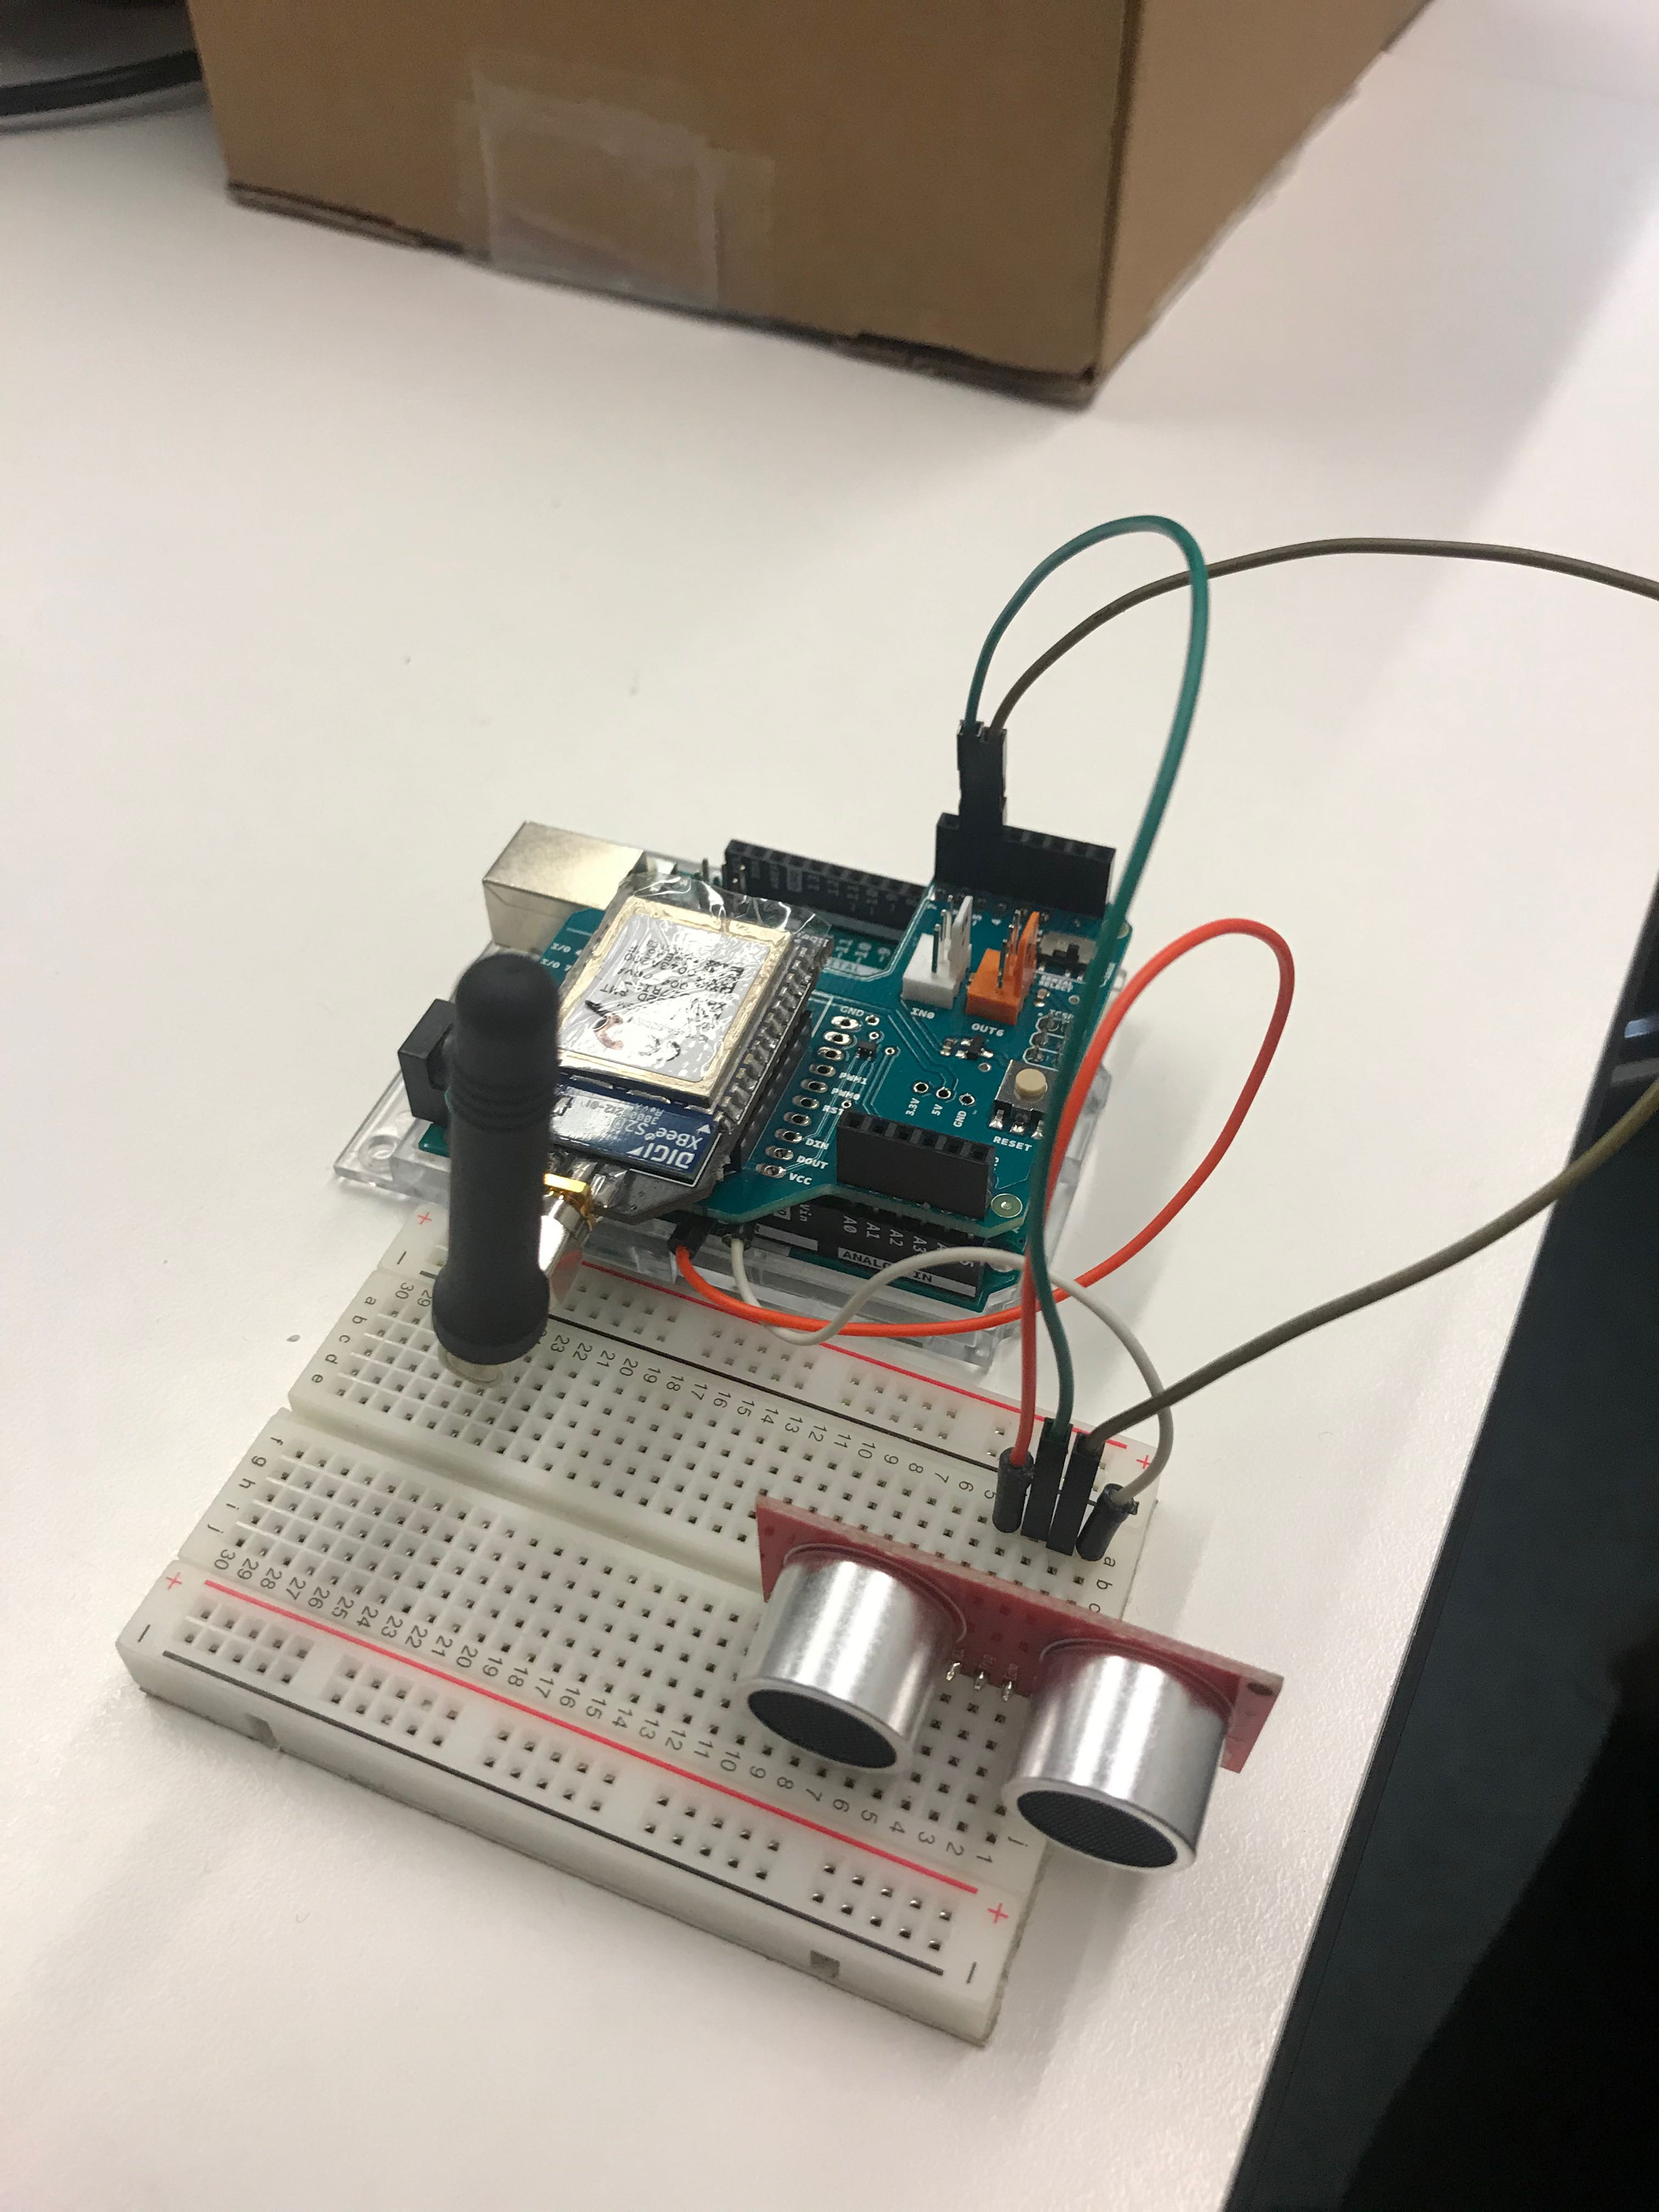
\includegraphics[width=\textwidth]{proximity.jpeg}
    \caption{Proximity sensor node}
    \label{fig:proximity}
\end{figure}
\FloatBarrier

\section{Software}
Our project has two kinds of IoT devices (based on sensors we got). We have the DHT22 (humidity and temperature) and HC-SR04 range finder. The IoT data is defined to be called as Telemetry. Telemetry is constructed from key (string), a value (float) and unit (string). We did this to have a unified format across all devices and protocols (listing \ref{telemetry}).

\begin{lstlisting}[language=C, caption=Message format, label=telemetry]
Class MessageFormat{
    public:
    struct Telemetry{
        String key;
        float value;
        String unit;
    };
}

\end{lstlisting}

DHT module works by using an external library on converting and querying info from sensors. It would have been a waste of time and really unnecessary to redevelop the basic tools. We used the Adafruits’ DHT.h -library. It has a simple function void DHT::begin that initiates the class, sets up pin modes and debug prints stuff for figuring out if something is wrong. We then gather the data separately as a DHT\_Message that is basically a struct that has humidity and temperature. The information is queried from the sensor through the library with methods dht.readHumidity() and dht.readTemperature(). 

Upon sending telemetry we obviously separate the temperature and humidity data into their own telemetry units. This is called controlled windowing. Since XBee library internals accept only an array of unsigned chars, we mask the data and compress it into the bare essentials of 5 chars (listing \ref{telemetry2}). 

\begin{lstlisting}[language=C, caption=Payload format, label=telemetry2]
//Payload is {hwid, t/h/p, tens, ones, unit}
unsigned char payload[5] = {0,0,0,0,0};
\end{lstlisting}

\section{Development environment}
We used general programming conducts and good guidelines. Our development is based mostly on Git versioning tool and is hosted on GitHub as a collaborative environment. We used both VSCode with Arduino extension and Arduino IDE to program the devices. For RF modules we used XCTU to flash and program their topology. We used several libraries, both internal and external and designed an appropriate folder structure (figure \ref{fig:folder}).

\begin{figure}[!htbp]
    \centering
    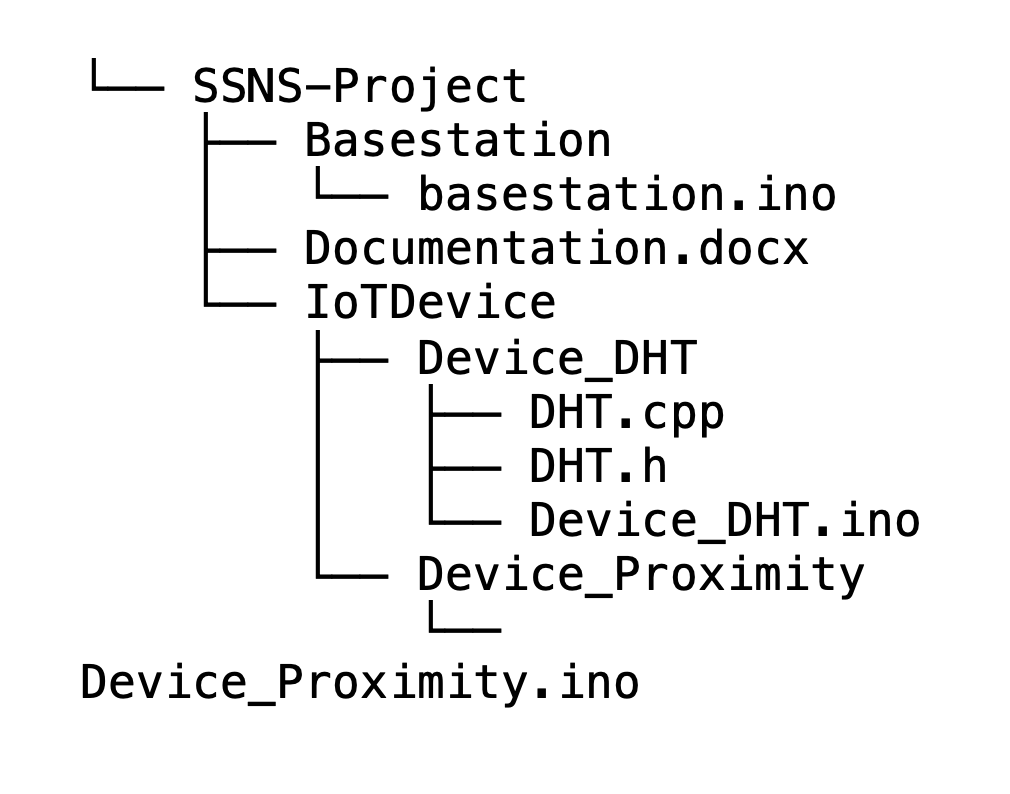
\includegraphics[width=\textwidth]{folder.png}
    \caption{Project folder structure}
    \label{fig:folder}
\end{figure}
\FloatBarrier

\section{Security}
XBee supports AES-128 symmetric encryption algorithm \cite{yussoff2010development} that is possible to configure using XCTU desktop application or just using serial connection with terminal emulator.  We discussed about the encryption of the communication on our project and we thought that our data is not sensitive at least not in this state. 


\chapter{Results}
\section{Showing data}
Our approach to showing the data to user is not very sophisticated. Although the scope of this program was to configure the node devices and the network not the user application. On our coordinator node we had a program that prints data to serial that XBee RF module receives from the sensor nodes. Easy way is to use terminal emulator to connect USB serial to the Arduino (listing \ref{console}). Proximity data is being sent every five second and environment conditions every 20 seconds.

It would have been nice to have some equipment with simple HTTP server and some logging function to save and show data in user friendly manner. For example ESP8266 with internet connection could have been used to send data to cloud based system using MQTT procotol. 

\begin{lstlisting}[language=bash, caption=User console, label=console]
#!/bin/bash
$ screen /dev/dev_coordinator 9600 
2p99c
3h22%
3t22C
4t23C
4p25%
\end{lstlisting}




\chapter{Implementation limitations and challenges}

\section{XBee}
We had challenges on configuring XBee S2D units because we did not have DIGI Explorer programming unit available. In order to configure XBee units we had to remove MCU from the Arduino because Arduino and XBee unist share the same usb serial connection. First we tried to connect to XBee units multiple times with no succes. Problem was that two XBee units were dead on arrival. We had to do our project with just four working radio modules which made our sensor network smaller than we wanted initially. 

\section{XBee library}
Second challenge was using the existing XBee library for Arduino boards. The issue was that the data was sent to coordinator as a unsigned char array. Because of that type limitation we had to do some type conversions on our Arduinos before sending data to XBee unit.

\section{Arduino with XBee shield}
We used XBee shield on top of the Arduino uno in order to connect XBee S2D unit. Challenge was that the XBee shield covered some GPIO pins that we initially wanted to use for our sensor communication. Other option would have been to solder sensor wires to XBee shield but that would have been an inconvenience for future users of the test bed devices. We managed to connect sensors to Arduino boards but it was not pretty and we had to bend some jumper wires. There was also a danger of short circuiting boards because of the close proximity of jumper wires and the traces of the XBee shield (see figure \ref{fig:proximity}).

% insert references
%  · included unsrtf.bst provides finnish language version of unsrt
\bibliographystyle{unsrtf}
\bibliography{References} % Oletustiedosto bibtex-viitteille. Halutessaan voi käyttää myös muita tapoja.

%%%%%%%%%%%%%%%%%%%%%%%%%%%%%%%%%%%%%%%%%%%%%%%%%%%%%%%%%%%%%%%%%%%%%%%%%%%
%
% Almost there....
%
%%%%%%%%%%%%%%%%%%%%%%%%%%%%%%%%%%%%%%%%%%%%%%%%%%%%%%%%%%%%%%%%%%%%%%%%%%%
\eofpages
\appendices

% create your appendix chapters with command \appchapter{some name} instead
% of \chapter{some name} for the automagic page counting to work

%\include{file name of appchapter xxx}
%\include{file name of appchapter yyy}
%\include{file name of appchapter zzz}
%\include{and so on}

%%%%%%%%%%%%%%%%%%%%%%%%%%%%%%%%%%%%%%%%%%%%%%%%%%%%%%%%%%%%%%%%%%%%%%%%%%%
%
% main document ends here
%
%%%%%%%%%%%%%%%%%%%%%%%%%%%%%%%%%%%%%%%%%%%%%%%%%%%%%%%%%%%%%%%%%%%%%%%%%%%
\eofapppages
\end{document}


